\documentclass{standalone}
\usepackage{tikz}
\usepackage{mathpazo}
\usetikzlibrary{shapes,snakes}

\definecolor{aiidaorange}{RGB}{255,124,22}
\definecolor{aiidagreen}{RGB}{48,184,7}
\definecolor{aiidablue}{RGB}{3,150,221}
\definecolor{marvelred}{RGB}{220,50,38}

\tikzstyle{box}=[draw, fill=aiidablue!30, minimum size=2em]
\tikzstyle{box-review}=[diamond, fill=aiidaorange!30, minimum size=2em]
\tikzstyle{box-implemented}=[draw, fill=aiidagreen!30, minimum size=2em]
\tikzstyle{box-negative}=[draw, fill=marvelred!30, minimum size=2em]
\tikzstyle{box-withdrawn}=[draw, fill=gray!30, minimum size=2em]

\begin{document}
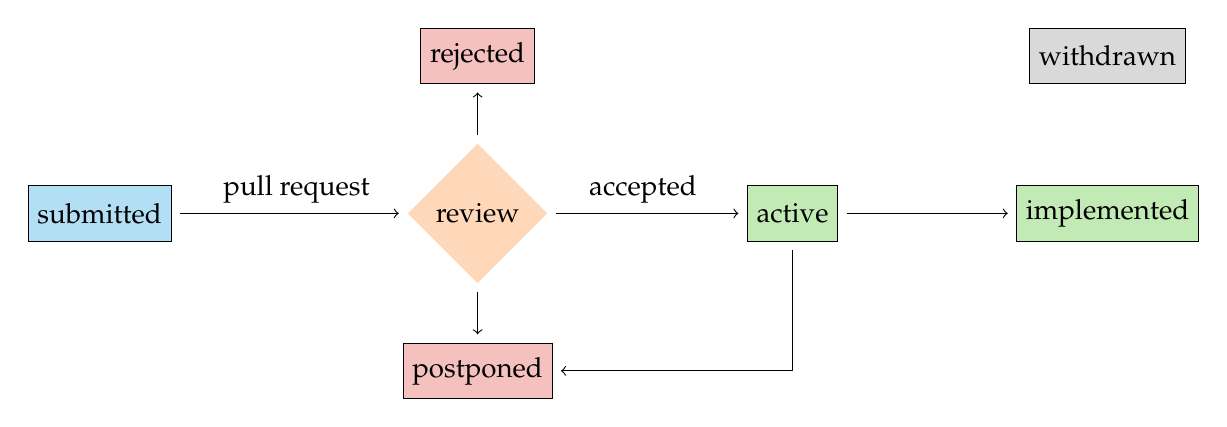
\begin{tikzpicture}
	% nodes
	 \node [box] (a) at (-0.8,0) {submitted};
	 \node [box-review] (b) at (4,0) {review};
	 \node [box-implemented] (c) at (8,0) {active};
	 \node [box-implemented] (d) at (12,0) {implemented};
	 \node [box-negative] (e) at (4,-2) {postponed};
	 \node [box-negative] (f) at (4, 2) {rejected};
	 
	 \node [box-withdrawn] (g) at (12, 2) {withdrawn};
	 
	 \node at (1.7,0.3) {pull request}; 
	 \node at (6.1,0.3) {accepted}; 
	  
	  
	 % arrows 
	 \draw [->, shorten >=3pt, shorten <=3pt] (a) -- (b); 
	 \draw [->, shorten >=3pt, shorten <=3pt] (b) -- (c); 
	 \draw [->, shorten >=3pt, shorten <=3pt] (b) -- (f);
	 \draw [->, shorten >=3pt, shorten <=3pt] (b) -- (e); 
	 \draw [->, shorten >=3pt, shorten <=3pt] (c) -- (d); 
	 
	 \draw [->, shorten >=3pt, shorten <=3pt] (c) -- (8,-2) -- (e);
	 	  
\end{tikzpicture}
\end{document}